%-----------------------------------------------------------------------------
%
%               Template for sigplanconf LaTeX Class
%
% Name:         sigplanconf-template.tex
%
% Purpose:      A template for sigplanconf.cls, which is a LaTeX 2e class
%               file for SIGPLAN conference proceedings.
%
% Author:       Paul C. Anagnostopoulos
%               Windfall Software
%               978 371-2316
%               paul@windfall.com
%
% Created:      15 February 2005
%
%-----------------------------------------------------------------------------


\documentclass[]{sigplanconf}

% The following \documentclass options may be useful:
%
% 10pt          To set in 10-point type instead of 9-point.
% 11pt          To set in 11-point type instead of 9-point.
% authoryear    To obtain author/year citation style instead of numeric.

\usepackage{graphicx}
\usepackage{amsmath}
\usepackage{hyperref}
\usepackage{graphicx}

\newcommand{\squishlist}{\begin{list}{$\bullet$}
  {\setlength{\itemsep}{0pt}
    \setlength{\parsep}{3pt}
    \setlength{\topsep}{3pt}
    \setlength{\partopsep}{0pt}
    \setlength{\leftmargin}{1.5em}
    \setlength{\labelwidth}{1em}
    \setlength{\labelsep}{0.5em}}}

\newcommand{\squishend}{\end{list}}

\begin{document}

\conferenceinfo{Sprezzatech}{Aug 6, Atlanta.} 
\copyrightyear{2013} 
\toappear{Copyright is held by the author.\\
\textit{Sprezzatech} Aug 6, Atlanta.}
%\authorpermission
%\titlebanner{CS8803DC, Spring 2010, Georgia Institute of Technology}        % These are ignored unless
%\preprintfooter{Dynamic Translation for Intel's Loop Stream Decoder}   % 'preprint' option specified.

\title{Streaming Audio in the Gulf of Guinea}
\subtitle{Categorizing and Delivering Nigeria's Music}

\authorinfo{Nick Black}
           {nick.black@sprezzatech.com}

\maketitle

\begin{abstract}
Nigeria presents unique challenges and opportunities to mobile internet streaming
services. Major services such as Pandora\cite{pandoracountries} and
Spotify\cite{spotifycountries} have no presence in West Africa. Its multiethnic
and vivid culture produced worldwide sensations: Chinua Achebe, Wole Soyinka,
Chris Ofili, and ``Nollywood'', the hub of African cinema. Nigeria
was recognized as a ``Next Eleven'' country by Goldman-Sachs\cite{n11},
and is predicted by \textit{The Economist} to be the world's third most-populous
nation by 2050\cite{economist}. Cellular penetration approaches 70\% of the population\cite{nigeriamobile},
provides 70\% of the nation's internet access, and is expected to increase
dramatically following the dissolution and sale of the moribund, state-run
NITEL (Nigeria Telecommunications, Limited)\cite{reutersnitel}. This cellular access,
however, suffers reliability, quality-of-service, and capability issues, with
many users adopting multiple carriers\cite{reuterssims}. Furthermore, nascent
Nigerian streamers such as iROKING and Gbedu.FM have not introduced 
automated classification.\\
\\
We investigate the technical issues of cost-effective streaming and
categorization of Nigerian music.
\end{abstract}

\category{ITU}{Region 1}{Nigeria}

\terms
Nigerian cellular, streaming music

\keywords
Nigeria, streaming, psychoacoustics

\section{Introduction}
Streaming music requires three technological capabilities:
\begin{itemize}
\item Bandwidth sufficient to deliver high-quality audio. The server side
	requires bandwidth for a great many concurrent streams: bandwidth
	requirements will generally follow the product of the number of streams
	and the streams' bit rates.
\item A delivery system capable of maintaining low jitter across the length
	of a song, and which does not introduce high latencies between songs.
\item The ability to categorize large amounts of music for the purposes of
	music discovery and automatic playlist generation. Music discovery
	is assisted by categorization refinement, while automatic playlist
	generation relies on very simple evaluations.
\end{itemize}
The first two capabilities are systematic, real-time quality-of-service
demands. The third can be performed offline, wholly on the server side.

\section{Telecommunications in Nigeria}
Nigerian Internet access is representative of West Africa and radically
distinct from that of North America and Europe.
\begin{itemize}
\item	\textbf{The majority of Nigeria's transnational traffic involves
	oceanic carriers.}
	Africa lacks a pan-continental ``backbone'' as measured by in-continent
	IXP (Internet eXchange Point) traffic\cite{pingdom}. IXPs are fragmented
	into three major hubs (South Africa, the East African islands, and
	Northern Africa); outside these hubs, few backbones cross national
	borders (the World Bank has extended a loan for the
	Central Africa Backbone Project, connecting ECCAS
	states\footnote{The Adaptable Program Loan (APL) for Phase 1 will
	connect three Economic Community of Central African members: Chad, Cameroon,
	and the Central African Republic\cite{apl1a}.}). Bandwidth
	into and out of Nigeria is thus paced by underwater cable laying, and
	subject to long-path latency. Nigeria has no true Tier 1 provider\footnote{The only
	Tier 1 ISPs in Africa operate from South Africa and Ghana\cite{drpeering}, though
	Suburban Telecom\cite{suburban}, Main One and Globanet all boast
	Tier 1 partners.}.
	
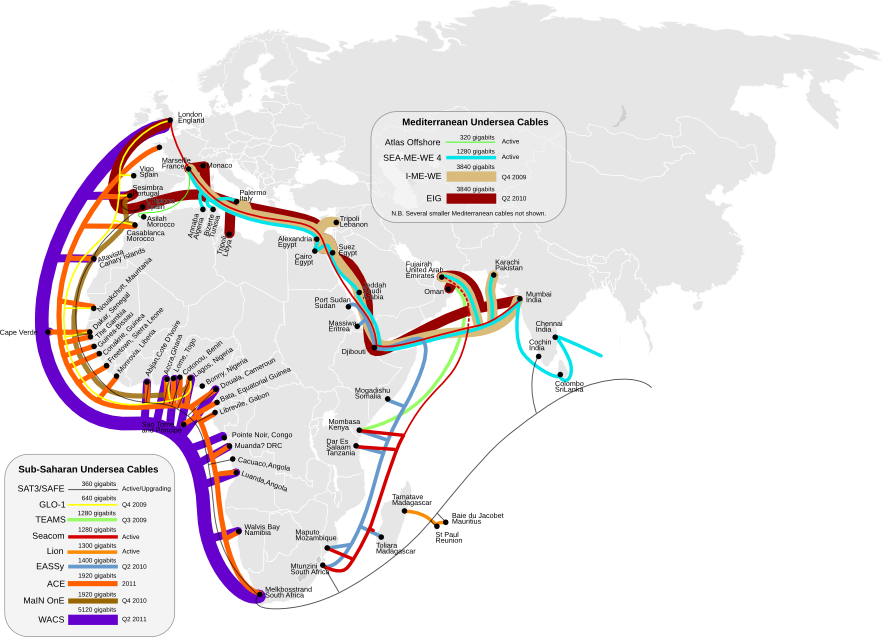
\includegraphics[scale=.4]{subsahara.png}

\item \textbf{The majority of Nigeria's intranational traffic involves
	cellular carriers.} Through 2009, international fiber bandwidth consisted solely of state monopoly
	NITEL's SAT-3/WASC access\cite{backbone}; reliability problems and cost drove 30\%
	of Internet users to high-latency, low-throughput
	Very Small Aperture Terminal (VSAT) parabolic satellite service.
	Numerous West African cables have since been added, including
	Globacom's Glo-1, MTN's Main One, Orange's ACE, and Alcatel-Lucent's WACS
	(Nigeria is not connected to ATLANTIS-2), with landing points at
	Lagos and Bonny Island. IXPN (formerly NIXP) offers 10Gbps IXPs at
	Lagos's NET House Colo and Vicroria Island's Medallian Colo\cite{ixpn}.
	Fiber backbones into the heart of Nigeria are underdeveloped; the NCC's
	Wire Nigeria Project and State Accelerated Broadband Initiative\cite{nccwire}
	aimed to subsidize development, but it is estimated that 40\% of Nigeria
	has no viable fixed access to national backbones\cite{biztech}.
	\\
	\\
	Widespread penetration of mobile devices thus preceded the development
	of major high-speed infrastructure in Nigeria. Like the cable internet
	providers that rose in the United States in the 2000's, end users
	already had last-mile connections by the time sufficient bandwidth and
	peering was available to provide them content. Unlike in America, the
	end users were connected by cellular radio.

\begin{figure}[h]
\centering
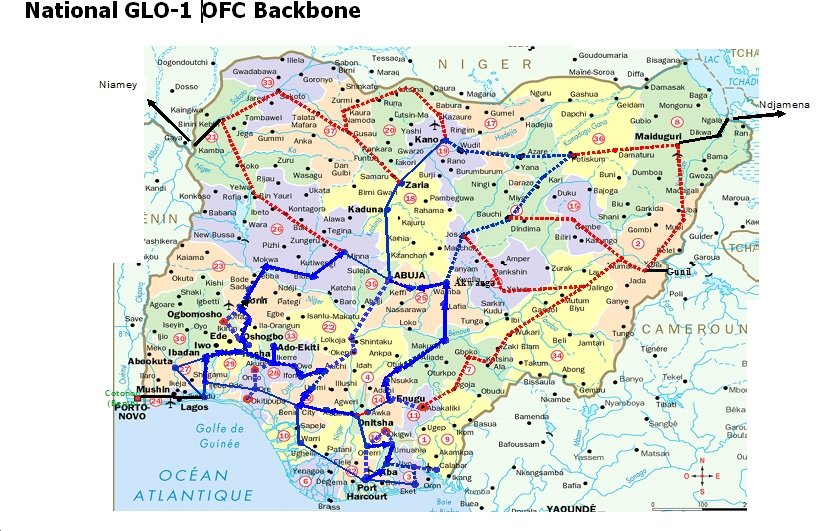
\includegraphics[width=\linewidth]{glo-1.jpg}
\caption{Globanet GLO-1 fiber network}
\end{figure}

\begin{figure}[h]
\centering
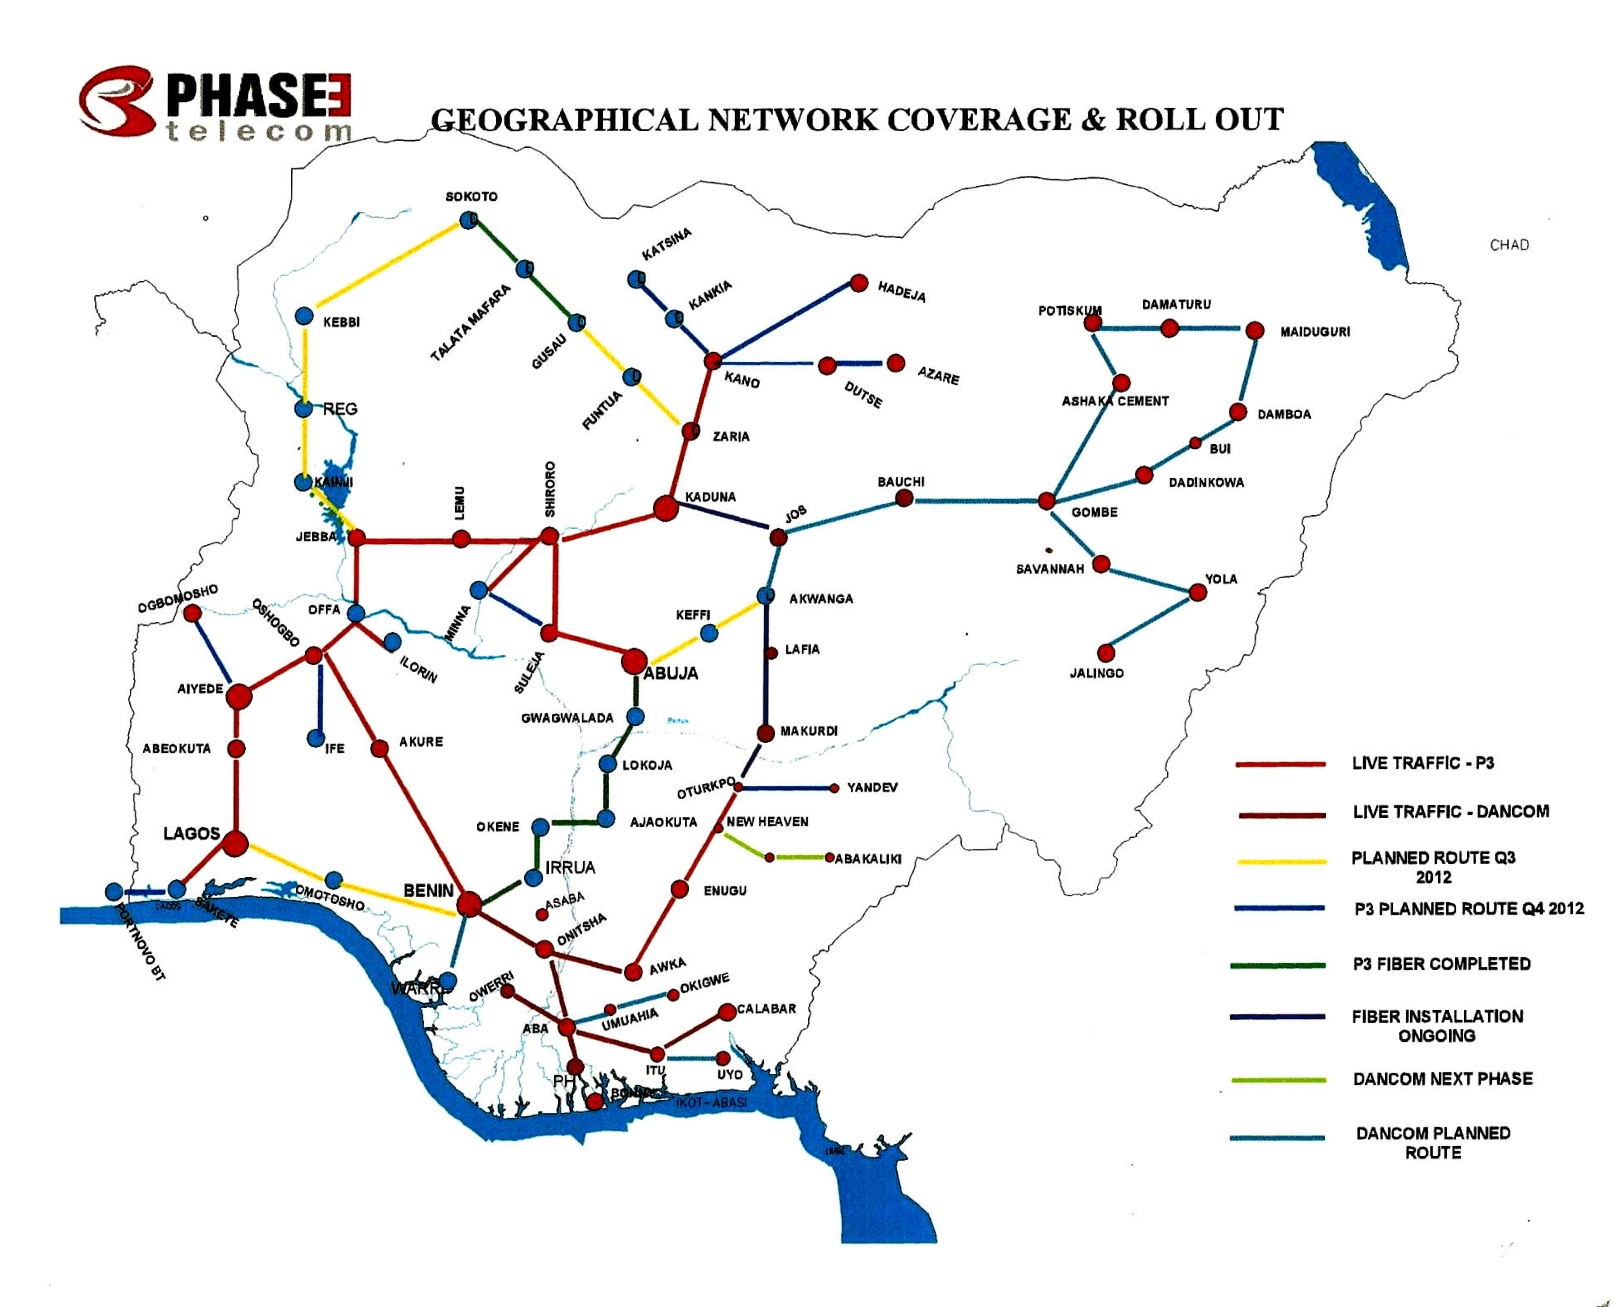
\includegraphics[width=\linewidth]{phase3.jpg}
\caption{Phase 3 fiber network}
\end{figure}

	The majority of Nigeria's fixed lines have been implemented using wireless technology\cite{fixedline}.
	Major ISPs position their mobile offerings ahead of their fixed ones (if
	the latter are indeed offered), and 70\% of Internet end users employ
	mobile on the last mile. Fixed WiMAX and 4G/LTE microwave links play
	critical backhaul roles where fiber and copper would typically be expected
	in North American and European networks\cite{wimax}. Hops within the
	country can be lossy, but don't tend to introduce much latency. The
	following \texttt{traceroute} output is indicative:

\begin{figure}[t]
\centering
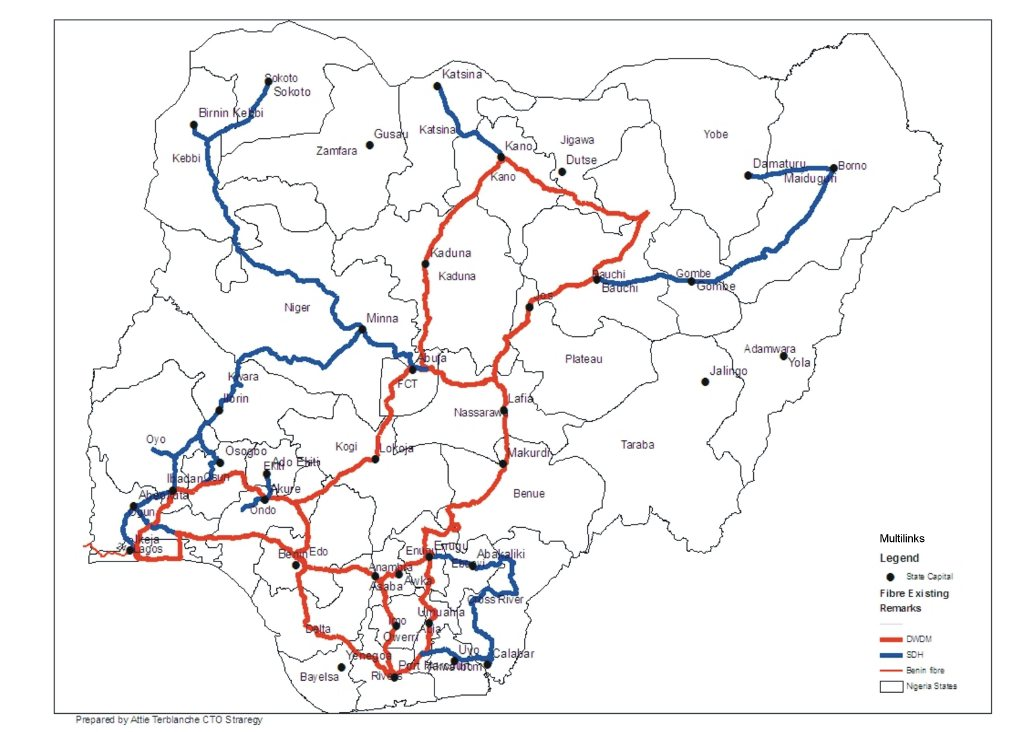
\includegraphics[width=\linewidth]{multilinks.jpg}
\caption{Multi-Links fiber network}
\end{figure}

\begin{figure}[t]
\centering
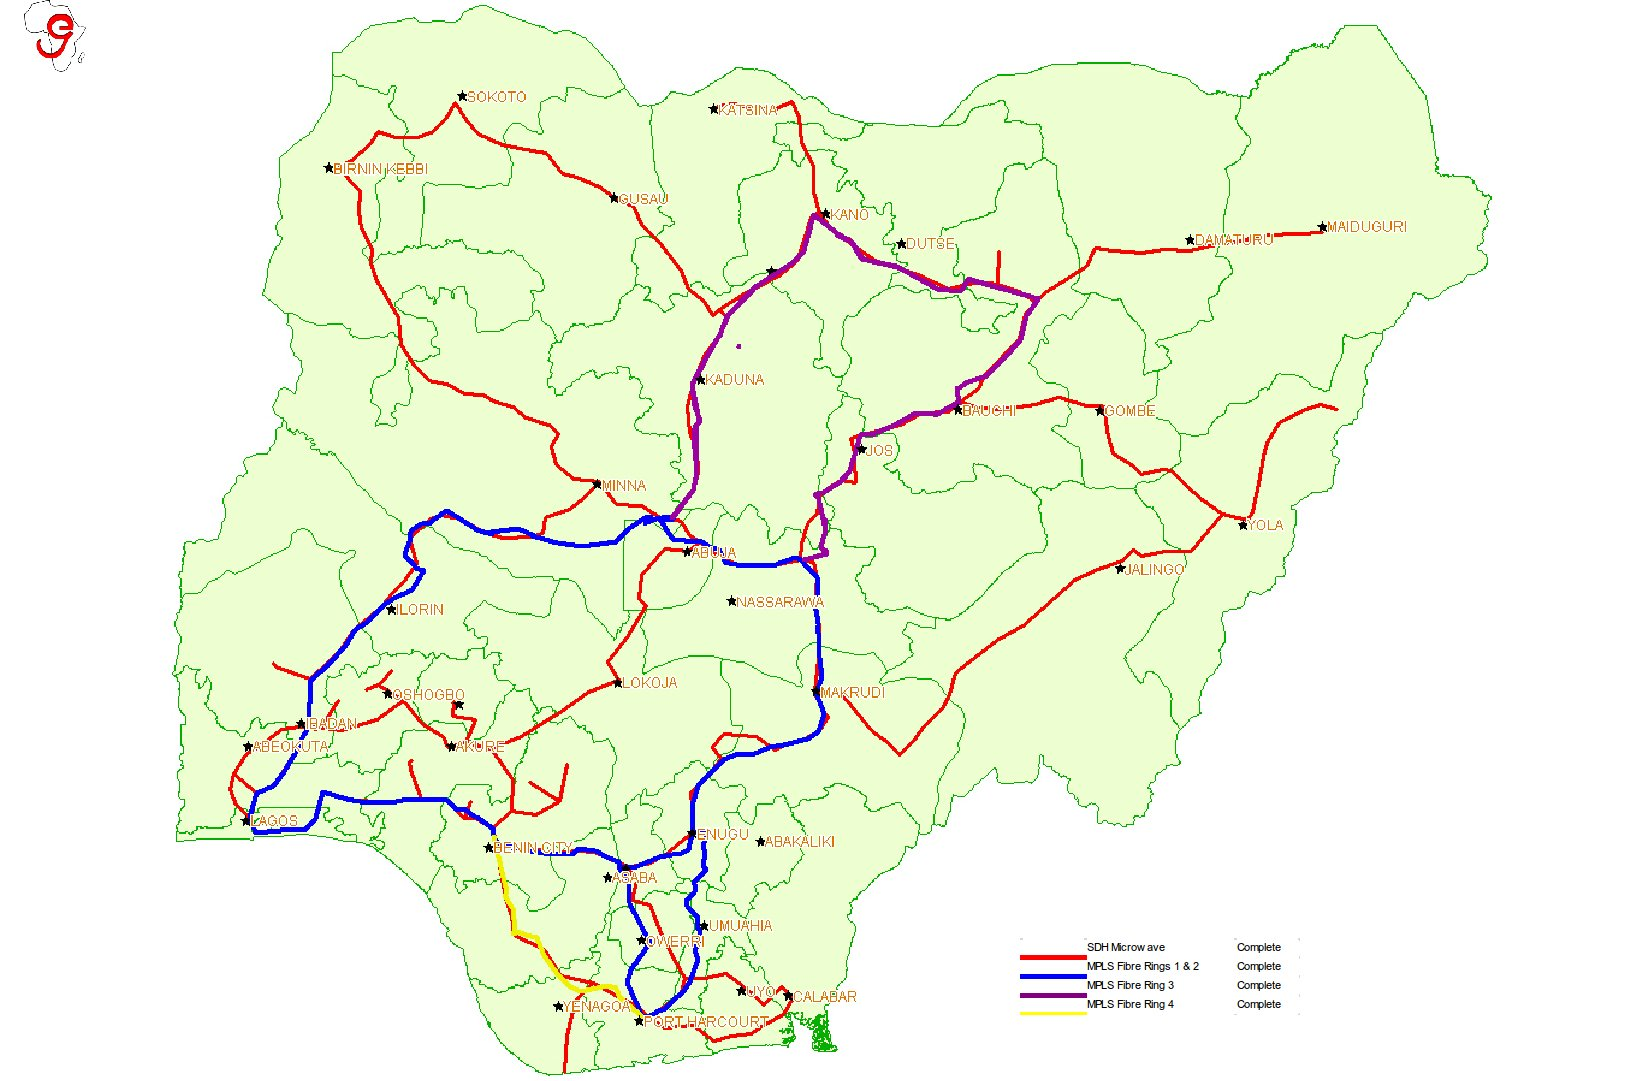
\includegraphics[width=\linewidth]{mtn.jpg}
\caption{MTN fiber network}
\end{figure}

	\begin{table}[h]
\begin{tabular}{ l | r | r | r | r }
	\textbf{Host} &
	\textbf{Last} &
	\textbf{Avg} &
	\textbf{Best} &
	\textbf{Worst} \\
\hline
z65-182-57-1.ips.direcpath.com & 0.4 & 0.5 & 0.4 & 1.3 \\
172.24.2.116 & 0.5 & 0.5 & 0.4 & 0.9 \\
172.24.0.246 & 0.5 & 0.7 & 0.4 & 1.3 \\
bboi-cbt.bboi.net & 0.5 & 0.5 & 0.5 & 0.6 \\
ash-ten3-1-atl-ten3-1.bboi.net & 14.6 & 15.6 & 14.5 & 32.2 \\
nj-ten2-2-ash-ten1-5.bboi.net & 19.6 & 24.5 & 19.4 & 39.3 \\
ny60-ten1-4-nj-ten2-1.bboi.net & 20.3 & 21.0 & 20.3 & 33.4 \\
lon-vl14-ny60-vl14.bboi.net & 108.2 & 114.8 & 99.8 & 155.0 \\
if-04.NG-CLS-PE-02.ngn.mainoneca & 186.8 & 186.8 & 186.7 & 187.0 \\
if-01.NG-POP-PE-01.ngn.mainoneca & 187.4 & 187.3 & 187.1 & 187.9 \\
41.75.84.166 & 191.4 & 191.5 & 191.0 & 194.8 \\
197.253.7.101 & 191.5 & 193.1 & 191.0 & 224.7 \\
\hline
\end{tabular}
\caption{Traceroute from Atlanta to Lagos}
\end{table}

The most latent hops here are, by far, the transatlantic jump from New Jersey
to London (Manasquan to Bude) over TAT-14's 1.87Tbps and the ride south over
the MTN Main One 1.28Tbps cable. Hops within Lagos are traversed with haste.
Several Nigerian servers selected from ProxyNova's database\cite{proxynova}
indicated \textasciitilde 10ms hops to Abuja (the capital) and major population
centers Kano and Kaduna.

\item \textbf{The vast majority of end-user access is made using mobile
devices.} Due to relatively low penetration of personal computers and DSL/cable
internet access (especially beyond major cities), 70\% of Nigerian internet
access points are mobile devices, and this number is expected to grow (mobile
device ownership is currently estimated by the ITU at 70\% of the population,
with many users employing multiple SIM cards):\\
\\
\\
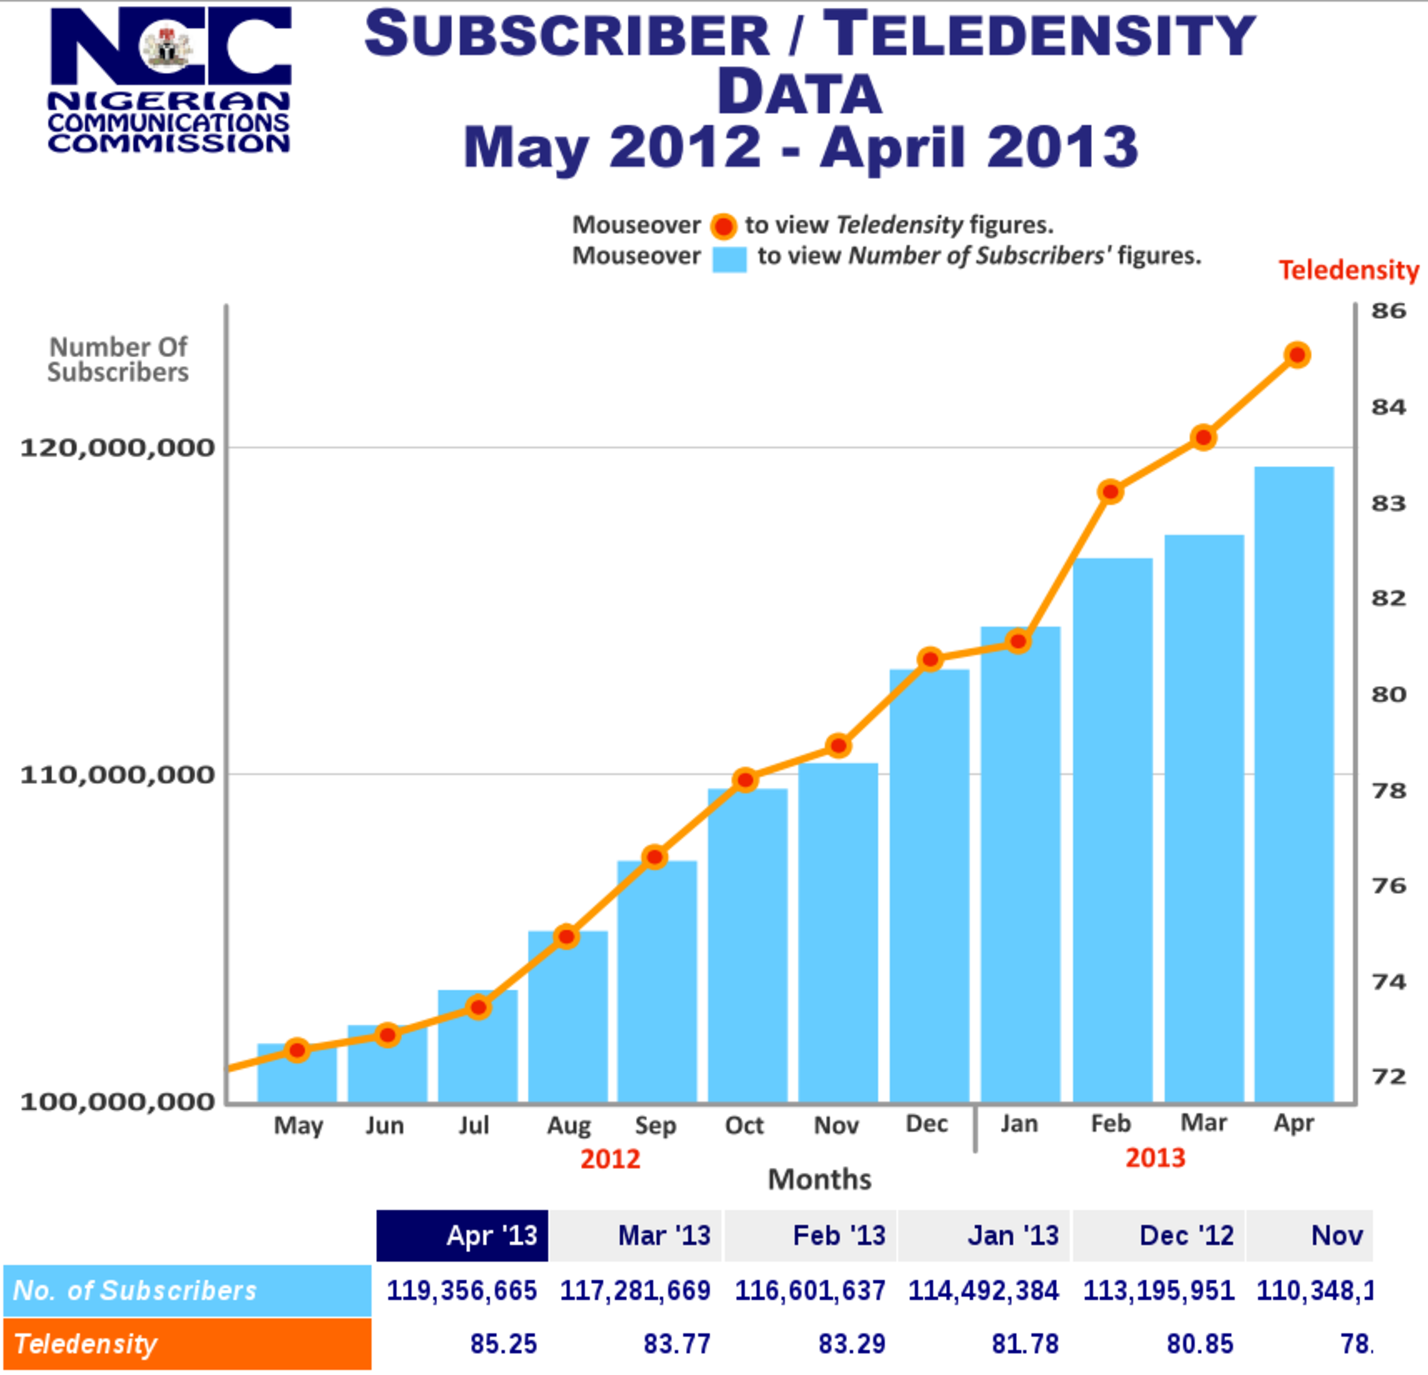
\includegraphics[width=\linewidth]{ncc.pdf}
\\
\\
According to the NCC, as of February 2013 mobile networks were dominated by
UMTS/HSDPA GSM (also known as 3.5G, 3G+ and ``turbo 3G''), making up
approximately 90 million of Nigeria's 128 mobile lines\footnote{MTN, GloMobile,
and Airtel offer UMTS/HSDPA GSM.}. Etisalat's basic 3G GSM connects another 15
million subscribers. CDMA/EVDO offerings make up the remaining 13
million\footnote{Visafone, Multilinks, Starcomms, and ZoomMobile offer
CDMA.}. The 32 million GPRS-provisioned internet accounts make up a
prevailing and growing majority of Nigerian packet switching.
\end{itemize}

What do these assessments imply?

\begin{itemize}
\item \textbf{Streaming media to Nigerian users requires a presence in Nigeria.}
Nigeria's relative paucity of international bandwidth and high-latency links to
major centers of computing confer strong advantages to distribution points
located in-country, despite a generally low level of technical education and
less competitive hosting economy.
\item \textbf{Successfully streaming media to Nigerian users does not imply
the ability to stream elsewhere.} For the same reason, Nigerian distribution
hubs cannot be expected to adequately provide streaming capability even to
other nations in the Gulf of Guinea. Successful completion of a West African
backbone, whether fiber, RoF (radio over fiber) or international 4G, would
greatly enhance transnational distribution from Nigeria, especially into Ghana.
\item \textbf{Sufficient bandwidth exists to stream music throughout Nigeria
from centralized facilities.} Latencies and packet drop rates within Nigeria's 
core national backbone are sufficiently low that edge-provisioning
is unlikely to significantly improve them. Redundancy (in the form
of sufficiently dense, independently-operated backbones) and short distances
overcome the need for multiple geographic emplacements. End-user bandwidth in
the 3G and 3G+ GSM networks is more than sufficient for streaming audio. The
major bandwidth chokeholds are likely to come along the fixed WiMAX backhaulage,
where decentralization is not likely capable of assisting distribution.
\item \textbf{Buffer at the end-user device; avoid realtime.} End users are
rich in bandwidth, but poor in reliability. It is likely that a connection the
length of a song will see bursty errors and, in some cases, loss of connection.
On the plus side, compressed audio typically requires less than 320Kbps (uncompressed
CD audio requires 1.5Mbps\footnote{2 channels * 44.1KHz * 16 bits = 1.411Mbps.}),
well below the multi-megabit rates of 3G+. Furthermore, modern smart phones provide
more than adequare RAM to store a complete song in memory.
\\
\\
The packet drop and jitter issues common to Nigeria's overprovisioned cellular
channels can thus be greatly ameliorated via bursty, full-speed transmission of
the stream (or even playlist), to be played back from the end user's device's
memory. Any bandwidth chokepoint will simply reduce burstiness, approaching
natural realtime delivery rates in the limit of bandwidth absolutely sufficient
for the stream\footnote{That is, if we can't get the bandwidth to play realtime,
delivery is screwed no matter what strategy you use.}. Aggregated over many
streams, this burstiness can of course be greatly augmented on the server side;
use of this strategy would be reckless without bandwidth controls on the server
uplink to avoid unexpected costs. These bandwidth controls will, of course,
require maintenance as demand scales, and such accounts might not comprete
pricewise. If a more realtime approach is desirable, UDP or some other unreliable
protocol is almost certainly suggested; should TCP be decided necessary,
it would be wise to employ SACK and run an appropriate TCP stack, though this
might only help on the server side\cite{tcp}.
\end{itemize}

\section{Provisioning for Streaming Music}
As noted above, CD-quality audio requires a theoretical maximum of 1.5Mbps
(open format FLAC lossless compression can reduce this by half, and lossy
compression can make further substantial reductions). We will work with
conservative figures: 5 minute lossless streams.
\begin{itemize}
\item \textbf{Storage}. Each stream requires 45MB of storage, assuming no
disk compression. An 8x2.5TB array can store thirty-three thousand
such streams using RAID6/RAID2Z or forty-four thousand when employed as JBOD 
(likely in the control of a cluster's distributed filesystem). Scaling to
several million songs, especially if compression is used, ought present no
difficulty.
\item \textbf{Disk bandwidth}. Assuming average sustained 50MBps reads, and
uniform access across disks, an 8-disk array can supply 3.2Gbps, sufficient
for twenty-one thousand concurrent unique 1.5Mbps streams.
\item \textbf{Controller bandwidth}. A SATA III 8-port controller ought be
able to drive 6Gbps, adequate for the 3.2Gbps input.
\item \textbf{PCIe bandwidth}. Assuming at least an 8-lane slot, PCIe 2.0
provides 4GBps, an order of magnitude more than is necessary.
\end{itemize}
Thus \textbf{network bandwidth effectively limits provisioning}. 1Gbps can
provide fewer than 700 uncompressed streams, which no machine ought have
problems handling. The bandwidth demand increases in proportion to the number
of streams and decreases in proportion to the effectiveness of any compression. 

\section{Automatic classification of music}
It is useful to distinguish between association and classification.
\begin{itemize}
\item \textbf{Association}. Two tracks $t_a, t_b$ are \textit{associated} under
some function $f(t)$ as $\frac{1}{| f(t_a) - f(t_b) | + 1}$. Given a current
track, and precomputed tables, it is trivial to find the $n$ most associated
tracks for any function. The difficulty is finding meaningful $f(t)$s. Some
are immediately obvious: ``Associate by exact album name match'', for instance,
can populate a playlist by reproducing an album\footnote{Assuming album
information is available.}. Some might rely on user feedback: ``Associate by
number of searches following playing this artist.''
\item \textbf{Classification}. A classification augments an association
via some schema by which $f(t)$ is made meaningful to a user.
\end{itemize}
Automated classification is not likely possible, outside a very few
associations. Automated association is possible to the degree $f(t)$ can
be automated. Automated discovery of associations is possible, but it might
not be possible to construct a meaningful classification from those
discovered. Automatic $f(t)$ come in four families:
\begin{itemize}
\item \textbf{Extracted acoustic data.} Open source tools exist purporting
to classify music via parametric analysis (e.g. beats per minute, volume
dynamics, instrument presence, or vocal pitch). The results can be stored and
compared to find associations. The question is: which associations are useful?
Do users want to search by vocal pitch? Which volume dynamics correspond to
dropping that bass?
\item \textbf{Cluster-matched data.} Machine learning approaches rely on a
training set to discover the best parametric analyses from some available set
by which to describe that training set. This can be very effective at finding
useful association functions, but meaningful classification will not
generally be possible. These tools are largely academic efforts, and their
quality ought be suspect until demonstrated.
\item \textbf{Other people's data.} Initial association discovery ought
crawl the resources of last.fm, AllMusic, Wikipedia, and other major music
databases. Top artists on last.fm's ``Nigeria'' channel include Fela Kuti,
P-Square, D'Banj, and 2face Idibia. New music must somehow be imported and
verified; is it too much to ask that basic classifications be provided as
part of the import package?
\item \textbf{User feedback.} At its simplest, this would correlate searches.
Feedbacks of arbitrary complexity are feasible, governed largely by front-end
development effort.
\end{itemize}
By a combination of these techniques, it ought be possible to implement at least
a limited-scope recommendation engine for many thousands of songs within a few
months. It will not be possible to trust this engine's accuracy without human
review, and it must be understood that substantial feedback and review will be
required for most automated schemes.

\section{Conclusions and Recommendations}
\begin{itemize}
\item Distribution can be run from a single point, ideally the NET House
Colocation Facility in Lagos. Distribution ought be performed from within
Nigeria. It should be understood that Nigeria is poorly-equipped to provision
beyond its borders, though this situation might change.
\item Network bandwidth will limit the number of streams that can be 
concurrently provided before hardware will.
\item Algorithmic classification of music can be performed, but will initially
need human review effort roughly equivalent to human classification effort.
Clustering is easier than classifying: it's easier to suggest something similar
to something else than it is to describe how they are similar, and providing
meaningful search capabilities is still more difficult.
\item Develop algorithmic classification from the beginning, but also expect
to perform classification by hand. This might pace the rate at which content
can be imported. Automated classification should thus be rolled out gradually;
launch can be done with only association, or even just search.
\item Initial association should be seeded, if possible, by scraping existing
databases. They ought also suggest classification schemata.
\item Even implicit user feedback can be effectively fed back for automated
associations.
\item Content licensing fees seem likely to dwarf technical costs.
\end{itemize}

\section{Moving Forward}
Sprezzatech is interested in bidding on construction and maintenance of
your computing resources in Nigeria, in concert with a competent local
agent of your specification. Sprezzatech is interested in bidding on design and
development of your music classification engine, and your delivery backend.\\
\\
Sprezzatech is not positioned to bid on development of your mobile frontend.\\
\\
Feel free to contact us with questions regarding this report.\\
\vspace{1in}\\
Nick Black, Principal

\vfill
\bibliographystyle{abbrvnat}
% The bibliography should be embedded for final submission.
\bibliography{nigeria}
\end{document}
